\documentclass[UTF8]{article}
\usepackage{ctex}
\usepackage{geometry}
\geometry{a4paper, scale=0.8}
\usepackage{graphicx}
\usepackage{subfigure}
\usepackage{float}
\usepackage{bookmark}
\usepackage{fontspec}
\newfontfamily\jetbrains{JetBrains Mono}
\usepackage{listings}
\usepackage{color}
\lstset{
    breaklines,                                 % 自动将长的代码行换行排版
    extendedchars=false,                        % 解决代码跨页时,章节标题,页眉等汉字不显示的问题
    backgroundcolor=\color[rgb]{0.96,0.96,0.96},% 背景颜色
    keywordstyle=\color{blue}\bfseries,         % 关键字颜色
    identifierstyle=\color{black},              % 普通标识符颜色
    commentstyle=\color[rgb]{0,0.6,0},          % 注释颜色
    stringstyle=\color[rgb]{0.58,0,0.82},       % 字符串颜色
    showstringspaces=false,                     % 不显示字符串内的空格
    numbers=left,                               % 显示行号
    numberstyle=\tiny\jetbrains,                    % 设置数字字体
    basicstyle=\small\jetbrains,                    % 设置基本字体
    captionpos=t,                               % title在上方(在bottom即为b)
    frame=single,                               % 设置代码框形式
    rulecolor=\color[rgb]{0.8,0.8,0.8},         % 设置代码框颜色
}
\usepackage{enumitem}
\usepackage{hyperref}
\hypersetup{
    hypertex=true,
    colorlinks=true,
    linkcolor=black,
    anchorcolor=black,
    citecolor=black
}
\usepackage{caption}
\usepackage{makecell}

\title{Verilog实验\ lab6实验报告}
\author{PB19071405\ 王昊元}
\date{2022 年 06 月 04 日}

\begin{document}
    \maketitle
    \section{实验目的}
    \begin{enumerate}
        \item 熟悉Tomasulo模拟器和cache一致性模拟器(监听法和目录法)的使用
        \item 加深对Tomasulo算法的理解,从而理解指令级并行的一种方式-动态指令调度
        \item 掌握Tomasulo算法在指令流出、执行、写结果各阶段对浮点操作指令以及load和store指令进行什么处理;
        给定被执行代码片段,对于具体某个时钟周期,能够写出保留站、指令状态表以及浮点寄存器状态表内容的变化情况
        \item 理解监听法和目录法的基本思想,加深对多cache一致性的理解
        \item 做到给出指定的读写序列,可以模拟出读写过程中发生的替换、换出等操作,同时模拟出cache块的无效、共享和独占态的相互切换
    \end{enumerate}
    \section{实验要求}
    \paragraph{Tomasulo算法模拟器}
    使用模拟器进行指令流的执行并对模拟器截图、回答问题
    \paragraph{多cache一致性算法-监听法}
    利用模拟器进行下述操作,填写下表,并截图,展示执行完以上操作后整个cache系统的状态。
    \paragraph{多cache一致性算法-目录法}
    利用模拟器进行下述操作,填写下表,并截图,展示执行完以上操作后整个cache系统的状态。
    \section{实验环境}
    \begin{itemize}
        \item 电三楼406机房电脑
        \item Windows 7
    \end{itemize}
    \section{实验结果及问题回答}
    \subsection{Tomasulo算法模拟器}
    \begin{enumerate}
        \item 分别截图(当前周期2和当前周期3),请简要说明load部件做了什么改动
        \begin{figure}[H]
            \centering
            \subfigure[当前周期2]{
                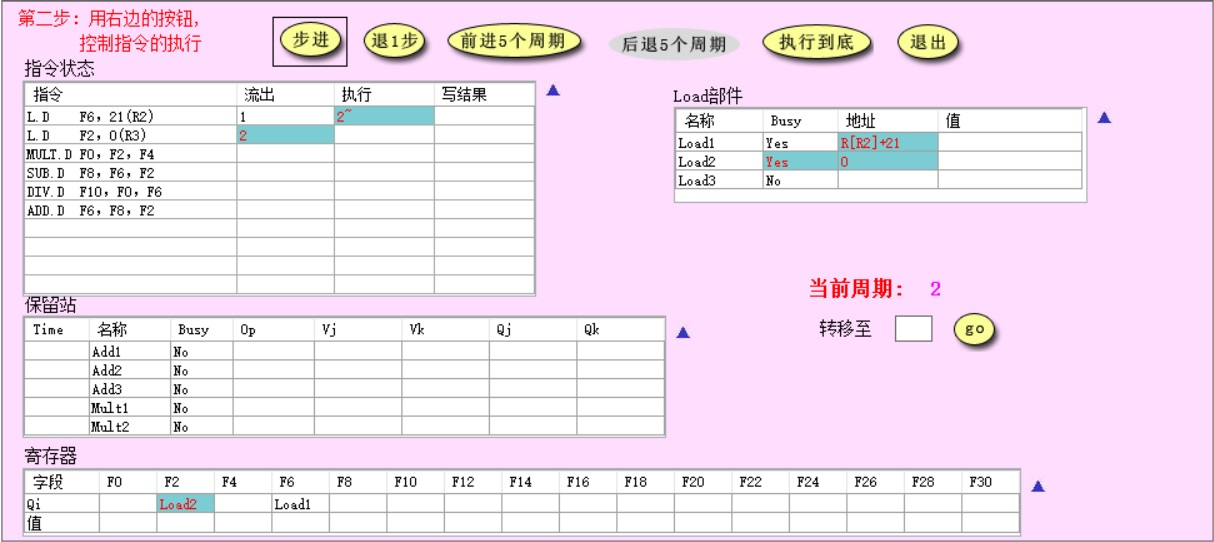
\includegraphics[width=0.4\textwidth]{./fig/tomasulo/cycle2.jpg}
            }
            \subfigure[当前周期3]{
                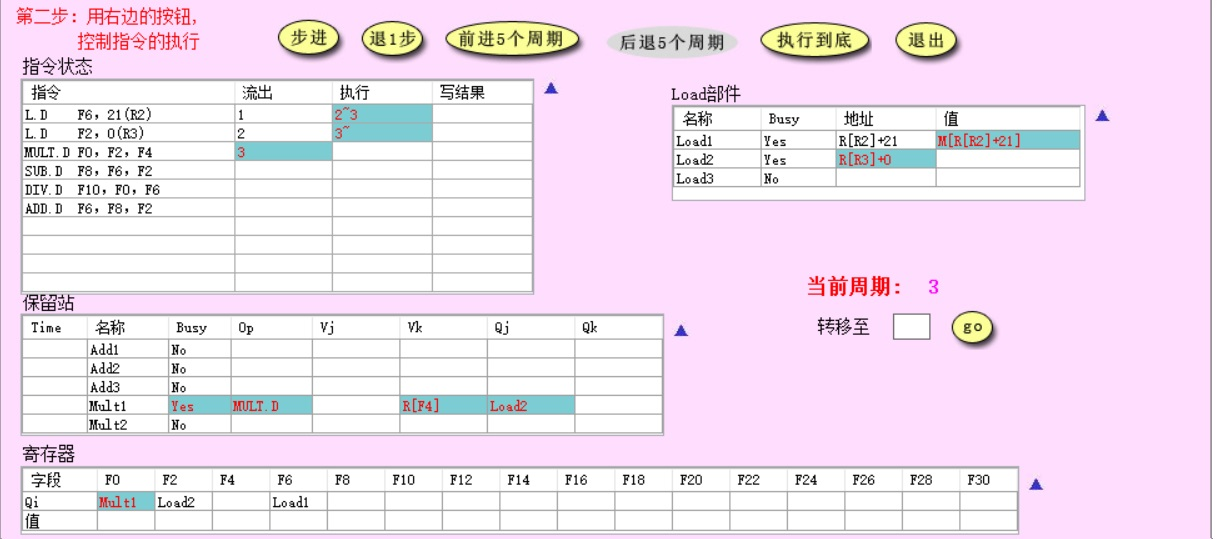
\includegraphics[width=0.4\textwidth]{./fig/tomasulo/cycle3.jpg}
            }
        \end{figure}
        \begin{enumerate}
            \item 对于当前周期2,Load2部件被占用,其Busy置为有效;存储器R2就绪,将偏移运算后的目标地址存于Load1部件的地址寄存器中。
            \item 对于当前周期3,Load1部件根据地址寄存器中地址,从存储器R2中对应的地址读取值至Load1部件的值寄存器中;存储器R3就绪,将偏移运算后的目标地址存于Load2部件的地址寄存器中。
        \end{enumerate}
        \item 请截图(MUL.D刚开始执行时系统状态),并说明该周期相比上一周期整个系统发生了哪些改动(指令状态、保留站、寄存器和Load部件)
        \begin{figure}[H]
            \centering
            \subfigure[MUL.D上一周期]{
                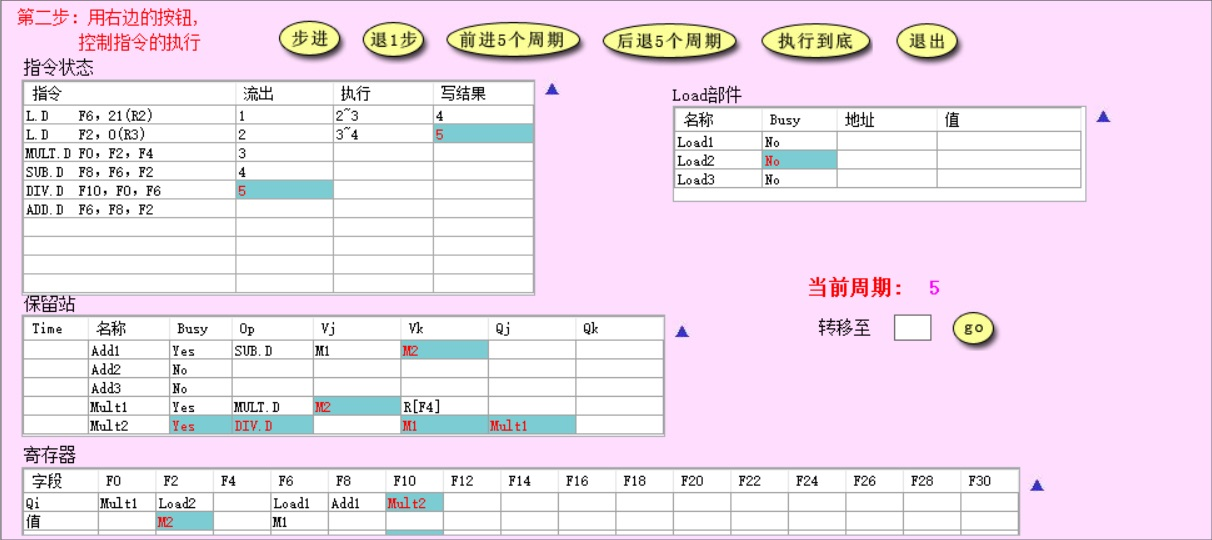
\includegraphics[width=0.4\textwidth]{./fig/tomasulo/before_muld.jpg}
            }
            \subfigure[MUL.D刚开始执行时的周期]{
                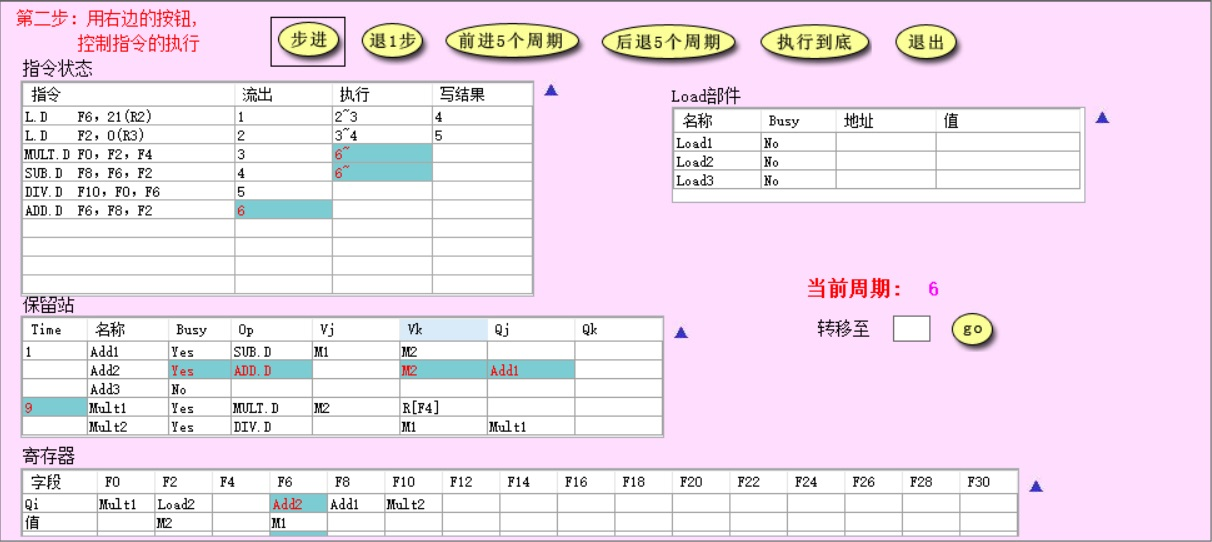
\includegraphics[width=0.4\textwidth]{./fig/tomasulo/muld.jpg}
            }
        \end{figure}
        \begin{itemize}
            \item 指令状态:第6条指令流出,第3、4条指令开始执行
            \item 保留站:新流出的第6条ADD.D类型的指令占用保留站Add2,第3条指令MUL.D和第4条指令SUB.D开始执行,同时二者各自的执行时间开始倒计时
            \item 寄存器:新发射的第6条ADD.D类型的指令等待F8寄存器就绪,准备向F6寄存器中写入值
            \item Load部件:无改动
        \end{itemize}
        \item 简要说明是什么相关导致MUL.D流出后没有立即执行 \\
        从第2条指令({\jetbrains L.D F2, 0(R3)})到第3条指令({\jetbrains MUL.D F0, F2, F4})间存在的关于F2的RAW相关导致MUL.D流出后没有立即执行,MUL.D需要等M2写入寄存器F2后才能执行。
        \item 请分别截图(15周期和16周期的系统状态),并分析系统发生了哪些变化
        \begin{figure}[H]
            \centering
            \subfigure[15周期]{
                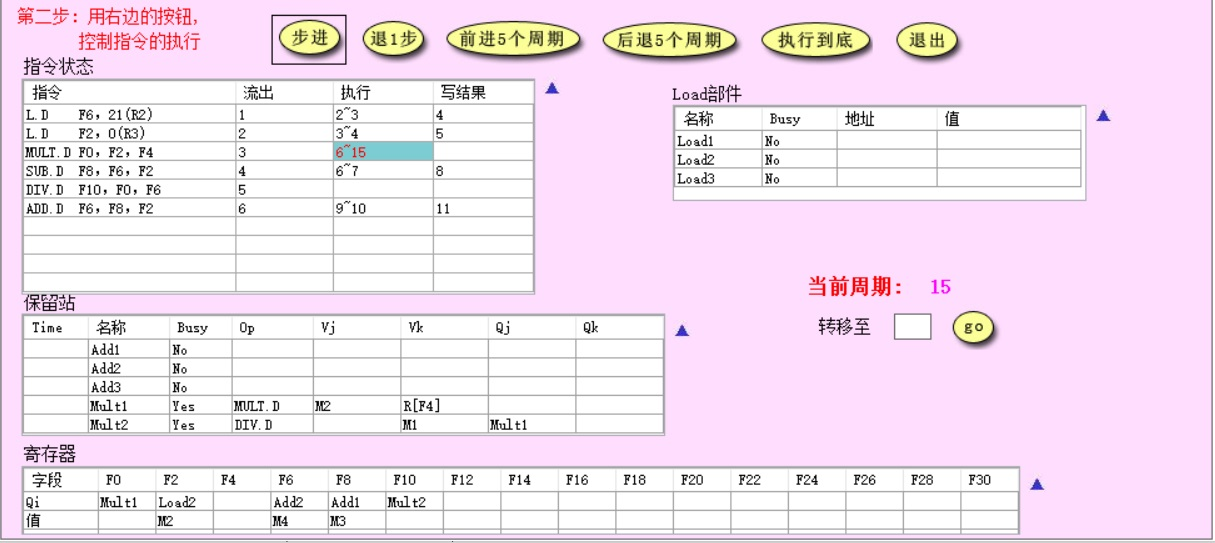
\includegraphics[width=0.4\textwidth]{./fig/tomasulo/cycle15.jpg}
            }
            \subfigure[16周期]{
                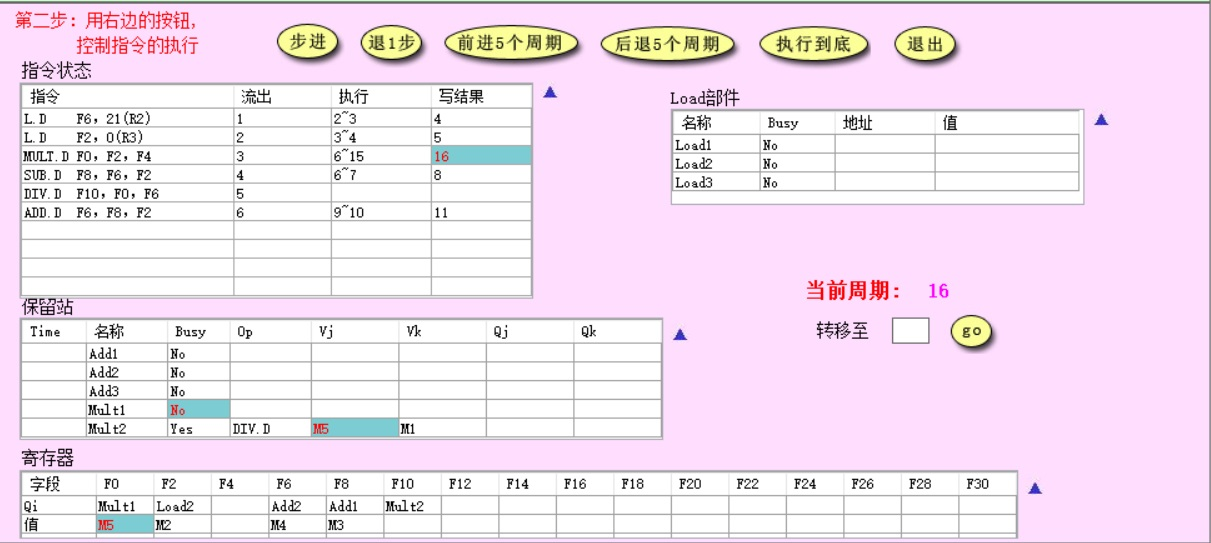
\includegraphics[width=0.4\textwidth]{./fig/tomasulo/cycle16.jpg}
            }
        \end{figure}
        \begin{enumerate}
            \item 第15周期:MULT.D执行完毕
            \item 第16周期:释放保留站Mult1,其Busy位置为无效;将指令MULT.D的结果M5写CBD,同时广播至寄存器F0和指令DIV.D对应的保留站Mult2
        \end{enumerate}
        \item 回答所有指令刚刚执行完毕时是第多少周期,同时请截图(最后一条指令写CBD时认为指令流执行结束) \\
        所有指令刚刚执行完毕时是第57个周期。
        \begin{figure}[H]
            \centering
            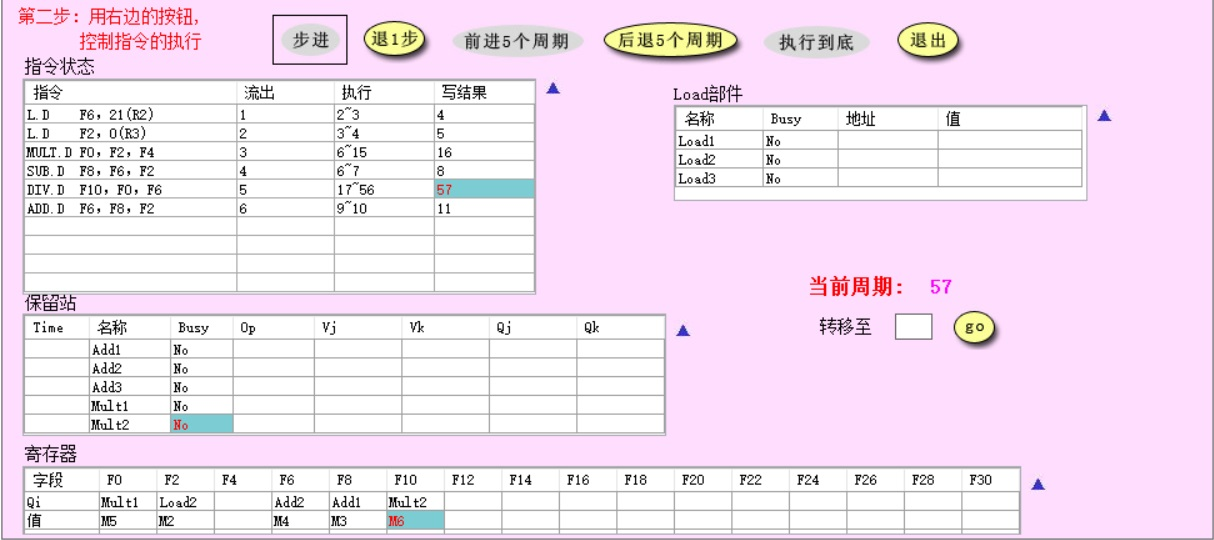
\includegraphics[width=0.7\textwidth]{./fig/tomasulo/end.jpg}
            \caption{所有指令刚刚执行完毕}
        \end{figure}
    \end{enumerate}

    \subsection{多cache一致性算法-监听法}
    \begin{table}[H]
        \centering
        \caption{监听法}
        \resizebox{\linewidth}{!}{
        % \begin{tabular}{c c c c}
        \begin{tabular}{c c c c}
            \hline
            所进行的访问 & \makecell[c]{是否发生\\了替换?} & \makecell[c]{是否发生\\了写回?} & 监听协议进行的操作与块状态改变 \\
            \hline
            \makecell[c]{CPU A\\读第5块} & 是 & 否 & \makecell[c]{Cache A发射Read Miss,存储器传输第5块到Cache A,\\替换Cache A的块1,Cache A的块1从状态I转为S对Cache A的块1进行读操作} \\
            \hline
            \makecell[c]{CPU B\\读第5块} & 是 & 否 & \makecell[c]{Cache B发射Read Miss,存储器传输第5块到Cache B,\\替换Cache B的块1,Cache B的块1从状态I转为S对Cache B的块1进行读操作} \\
            \hline
            \makecell[c]{CPU C\\读第5块} & 是 & 否 & \makecell[c]{Cache C发射Read Miss,存储器传输第5块到Cache C,\\替换Cache C的块1,Cache C的块1从状态I转为S对Cache C的块1进行读操作} \\
            \hline
            \makecell[c]{CPU B\\读第5块} & 否 & 否 & \makecell[c]{Cache B发射Invalidate,Cache A的块1从状态S转换到I,\\Cache C的块1从状态S转换到I,对Cache B的块1进行写操作,Cache B的块1从状态S转换到M} \\
            \hline
            \makecell[c]{CPU D\\读第5块} & 是 & 是 & \makecell[c]{Cache D发射Read Miss,写回Cache B的块1至存储器的第5块,\\Cache B的块1从状态M转为S,存储器传输第5块到Cache D,\\替换Cache D的块1,Cache D的块1从状态I转为S对Cache D的块1进行读操作} \\
            \hline
            \makecell[c]{CPU B\\读第21块} & 是 & 否 & \makecell[c]{Cache B发射Write Miss,存储器传输第21块到Cache B,\\替换Cache B的块1,Cache B的块1从状态S转换为M,对Cache B的块1进行写操作} \\
            \hline
            \makecell[c]{CPU A\\读第23块} & 是 & 否 & \makecell[c]{Cache A发射Write Miss,存储器传输第23块到Cache A,\\替换Cache A的块3,Cache A的块3从状态I转换为M,对Cache A的块3进行写操作} \\
            \hline
            \makecell[c]{CPU C\\读第23块} & 是 & 是 & \makecell[c]{Cache C发射Write Miss,写回Cache A的块3至存储器的第23块,\\Cache A的块3从状态M转为I,存储器传输第23块到Cache C,\\替换Cache C的块3,Cache C的块3从状态I转为M,对Cache C的块3进行写操作} \\
            \hline
            \makecell[c]{CPU B\\读第29块} & 是 & 是 & \makecell[c]{写回Cache B的块1至存储器的第21块,Cache B的块1从状态M转换为I,\\Cache B发射Read Miss,存储器传输第29块到Cache B,\\替换Cache B的块1,Cache B的块1从状态I转换为S对Cache B的块1进行读操作} \\
            \hline
            \makecell[c]{CPU B\\读第5块} & 是 & 否 & \makecell[c]{Cache B发射Write Miss,存储器传输第5块到Cache B,替换Cache B的块1,\\Cache B的块1从状态S转换为M,Cache D的块1从状态S转换为I,对Cache B的块1进行写操作} \\
            \hline
        \end{tabular}
        }
    \end{table}
    \begin{figure}[H]
        \centering
        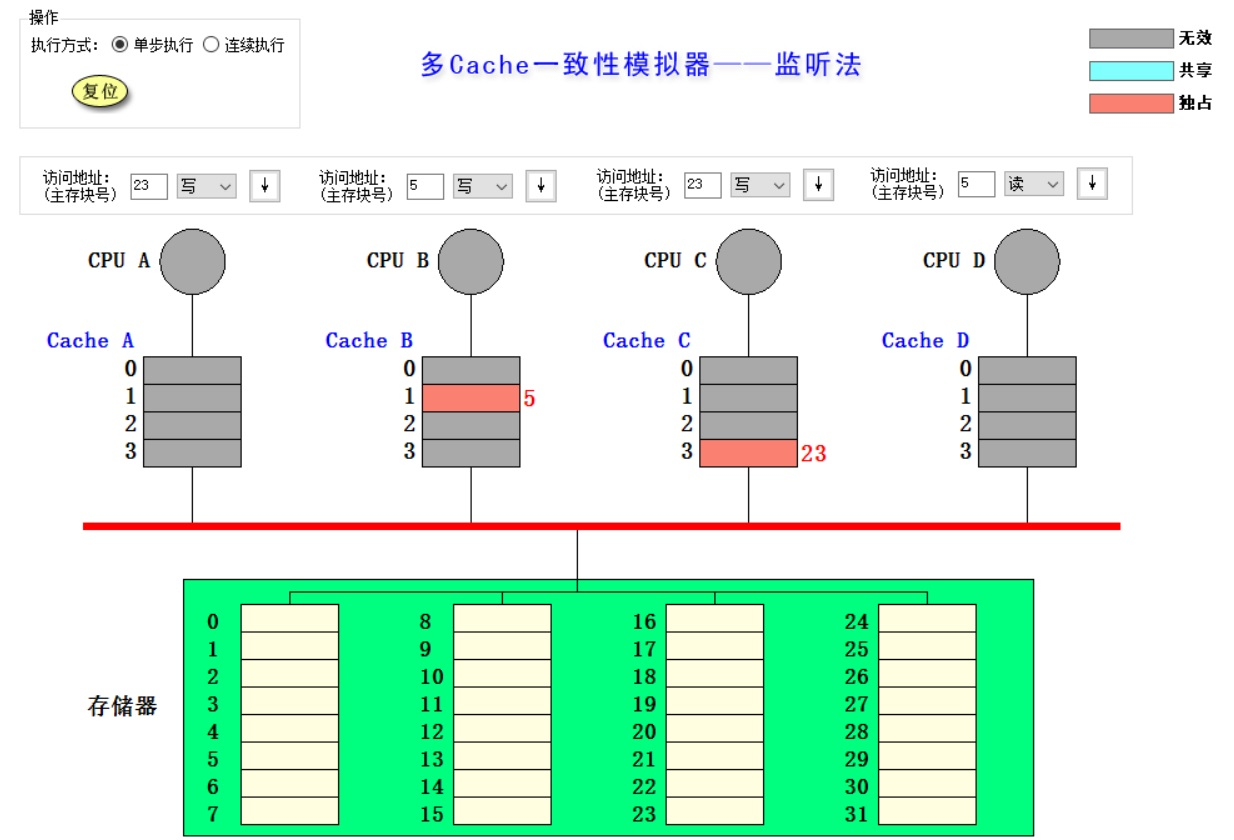
\includegraphics[width=0.7\textwidth]{./fig/snooping/end.jpg}
        \caption{监听法执行完后的状态}
    \end{figure}

    \subsection{多cache一致性算法-目录法}
    \begin{table}[H]
        \centering
        \caption{目录法}
        \resizebox{\linewidth}{!}{
        \begin{tabular}{cc}
            \hline
            所进行的访问 & 监听协议进行的操作与块状态改变 \\
            \hline
            \makecell[c]{CPU A\\读第6块} & \makecell[l]{Cache A发射Read Miss到Memory A,Memory A传输第6块到Cache A,替换Cache A的块2,\\Cache A的块2从状态I转为S;\\Memory A的块6由状态U转为S,其Presence bits由0000变为0001,其共享集合变为\{A\};\\对Cache A的块2进行读操作} \\
            \hline
            \makecell[c]{CPU B\\读第6块} & \makecell[l]{Cache B发射Read Miss到Memory A,Memory A传输第6块到Cache B,替换Cache B的块2,\\Cache B的块2从状态I转为S;\\Memory A的块6状态仍为S,Presence bits由0001变为0011,共享集合变为\{A,B\};\\对Cache B的块2进行读操作} \\
            \hline
            \makecell[c]{CPU D\\读第6块} & \makecell[l]{Cache D发射Read Miss到Memory A,Memory A传输第6块到Cache D,替换Cache D的块2,\\Cache D的块2从状态I转为S;\\Memory A的块6状态仍为S,Presence bits由0011变为1011,共享集合变为\{A,B,D\};\\对Cache D的块2进行读操作} \\
            \hline
            \makecell[c]{CPU B\\读第6块} & \makecell[l]{Cache B发射Write Hit到Memory A,Memory A发射Invalidate(6)到Cache A和Cache D,\\Cache A的块2从状态S转为I,Cache D的块2从状态S转为I,Cache B的块2从状态S转为M;\\Memory A的块6由状态S转为M,Presence bits由1011变为0010,共享集合变为\{B\};\\对Cache B的块2进行写入} \\
            \hline
            \makecell[c]{CPU C\\读第6块} & \makecell[l]{Cache C发射Read Miss到Memory A,Memory A发送Fetch(6)到Cache B,\\Cache B传输第6块到Memory A,Cache B的块2从状态M转为S,\\Memory A传输第6块到Cache C,替换Cache C的块2,\\Cache C的块2从状态I转为S;\\Memory A的块6由状态M转为S,Presence bits由0010变为0110,共享集合变为\{B,C\};\\对Cache C的块2进行读操作} \\
            \hline
            \makecell[c]{CPU D\\读第20块} & \makecell[l]{Cache D发射Write Miss到Memory C,\\Memory C传输第20块到Cache D,替换Cache D的块0,Cache D的块0从状态I转为M;\\Memory C的块20由状态U转为M,Presence bits由0000变为1000,共享集合变为\{D\};\\对Cache D的块0进行写入} \\
            \hline
            \makecell[c]{CPU A\\读第20块} & \makecell[l]{Cache A发射Write Miss到Memory C,Memory C发送Fetch\&Invalidate(20)到Cache D,\\Cache D传输第20块到Memory C,Cache D的块0从状态M转为I,\\Memory C传输第20块到Cache A,替换Cache A的块0,Cache A的块0从状态I转为M;\\Memory C的块20状态仍为M,Presence bits由1000变为0001,共享集合变为\{A\};\\对Cache A的块0进行写入} \\
            \hline
            \makecell[c]{CPU D\\读第6块} & \makecell[l]{Cache D发射Write Miss到Memory A,Memory A发射Invalidate(6)到Cache B和Cache C,\\Cache B的块2从状态S转为I,Cache C的块2从状态S转为I,\\Memory A传输第6块到Cache D,替换Cache D的块2,Cache D的块2从状态I转为M;\\Memory A的块6由状态S转为M,Presence bits由0110变为1000,共享集合变为\{D\};\\对Cache D的块2进行写入} \\
            \hline
            \makecell[c]{CPU A\\读第12块} & \makecell[l]{Cache A发送Write Back到 Memory C,Cache A的块0从状态M转为I,Cache A发射Read Miss到Memory B,\\Memory B传输第12块到Cache A,替换Cache A的块0,Cache A的块0从状态I转为S;\\Memory C的块20由状态M转为U,其Presence bits由0001变为0000,其共享集合变为$\emptyset$;\\Memory B的块12由状态U转为S,其Presence bits由0000变为0001,其共享集合变为\{A\};\\对Cache A的块0进行读操作} \\
            \hline
        \end{tabular}
        }
    \end{table}
    \begin{figure}[H]
        \centering
        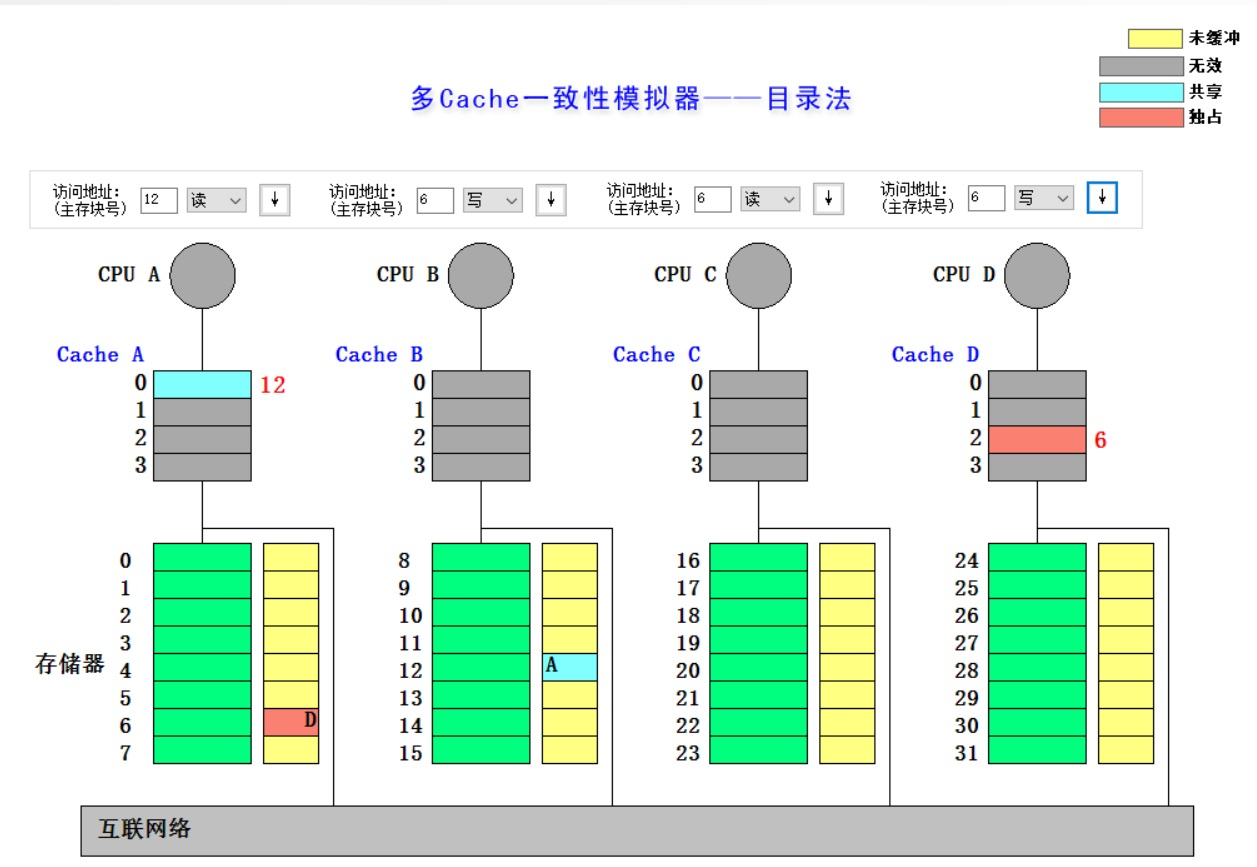
\includegraphics[width=0.7\textwidth]{./fig/directory/end.jpg}
        \caption{目录法执行完后的状态}
    \end{figure}
    \section{综合问答}
    \begin{enumerate}
        \item 目录法和监听法分别是集中式和基于总线,两者优劣是什么?(言之有理即可)
        \begin{enumerate}
            \item 监听法
            \begin{itemize}
                \item 优点
                \begin{itemize}
                    \item 保证了 Cache 的一致性,实现了写互斥和写串行
                \end{itemize}
                \item 缺点
                \begin{itemize}
                    \item 存在总线竞争问题
                    \item 总线事务多,通信开销大
                    \item 总线的带宽受限
                    \item 扩展性差,总线上能够连接的处理器数目有限
                    \item 在非总线和或环形网络上监听困难
                \end{itemize}
            \end{itemize}

            \item 目录法
            \begin{itemize}
                \item 优点
                \begin{itemize}
                    \item 降低了对于总线带宽的占用
                    \item 拓展性强,可以连接的处理器数目更多
                    \item 可以有效地适应交换网络进行通信
                \end{itemize}
                \item 缺点
                \begin{itemize}
                    \item 存在总线竞争问题
                    \item 需要额外的空间来存储 Presence Bits,当处理器数目较多的时,存储开销较大
                    \item 存储器接口通信压力大,存储器速度限制传输速度
                \end{itemize}
            \end{itemize}
        \end{enumerate}
        \item Tomasulo算法相比Score Board算法有什么异同?(简要回答两点:1.分别解决了什么相关,2.分别是分布式还是集中式)(参考第五版教材)
        \begin{itemize}
            \item Tomasulo算法为分布式;其指令状态、相关控制和操作数缓存分布在各个部件中(保留站)。其核心思想是:记录和检测指令相关,操作数一旦就绪就立即执行。把发生RAW(写后读)冲突的可能性减少到最少;通过寄存器换名来消除WAR(读后写)和WAW(写后写)冲突;指令若存在结构冲突,则不予以发射。
            \item Score Board算法为集中式;其不能解决WAR和WAW相关,只能检测到WAR和WAW相关,它是通过将后一条指令暂停来克服此类问题的。
        \end{itemize}
        \item Tomasulo算法是如何解决结构、RAW、WAR和WAW相关的?(参考第五版教材)
        \begin{itemize}
            \item 结构相关:有结构冲突不发射
            \item RAW相关:等待至写入完成,待读取的寄存器中的数据就绪,冲突消除后,再进入读指令执行阶段
            \item WAW相关:使用RS中的寄存器值或指向RS的指针代替指令中的寄存器-寄存器重命名
            \item WAR相关:使用RS中的寄存器值或指向RS的指针代替指令中的寄存器-寄存器重命名
        \end{itemize}
    \end{enumerate}
    % \section{实验总结}
    % \begin{enumerate}
    %     \item 
    % \end{enumerate}
\end{document}